\chapter{Methodology}
    \section{Controller Design}
    Two separate controllers were used in this research. The first controller is a low-level path-following controller recreated from the literature that maps input states to motor RPMs \cite{Mokhtar}. Fig. \ref{mokhtar_cont} shows a block diagram of the controller.
    \begin{figure}[H]
            \centering
            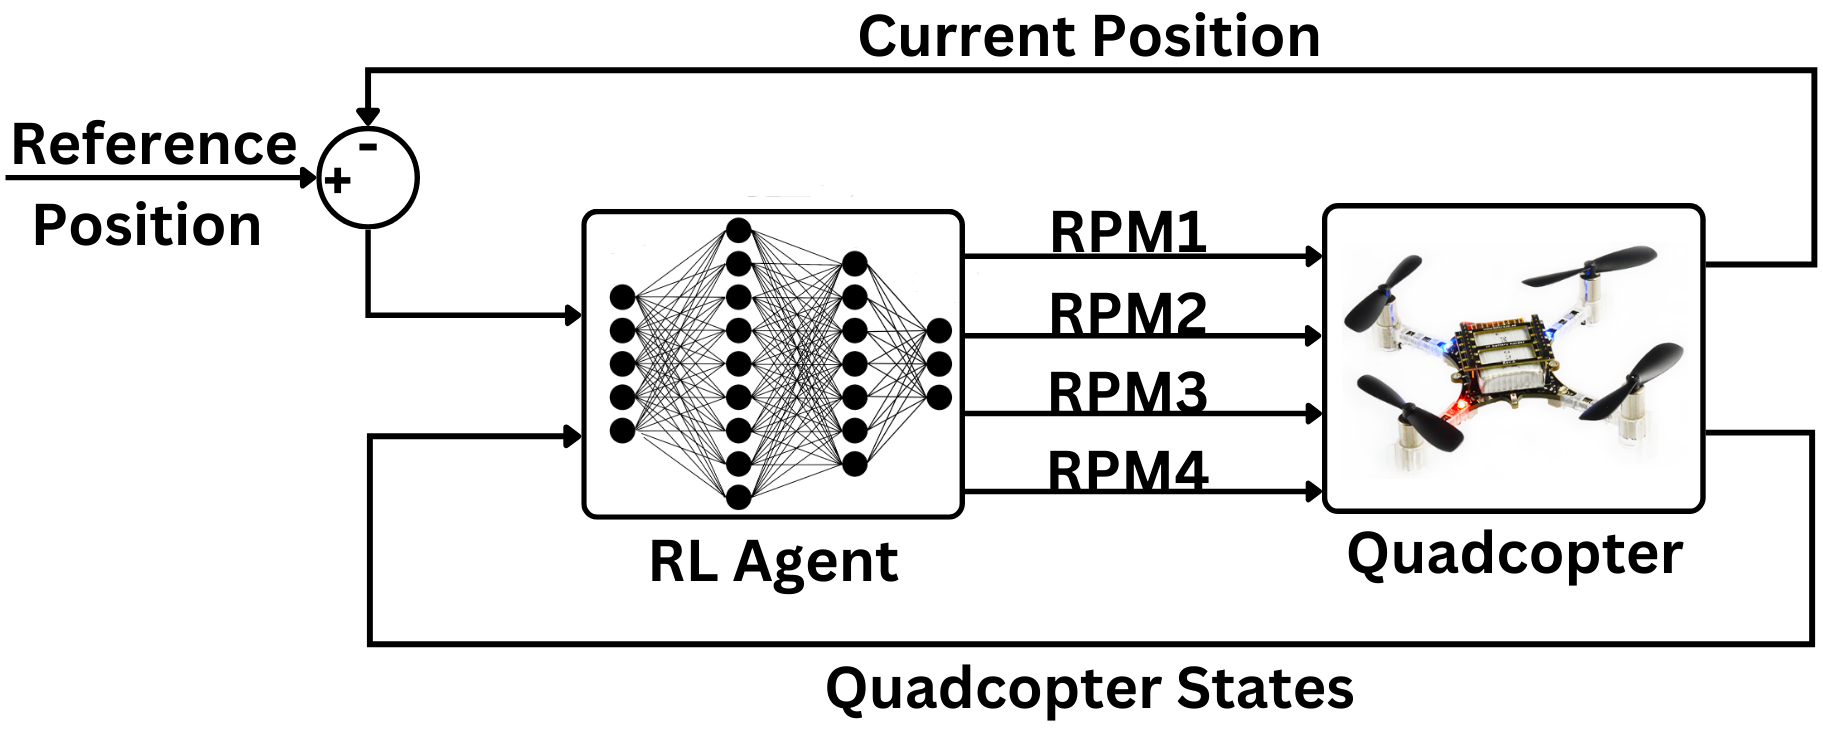
\includegraphics[width=0.8\linewidth]{Images/mokhtar.png}
            \caption{Block Diagram of the Path-following Controller for the Quadcopter}
            \label{mokhtar_cont}
    \end{figure}
    The agent takes as an input the position error and the current state of the drone and outputs four RPM signals for the four motors of the quadcopter.\clearpage
    The second controller used is a position controller that maps the input states into the desired roll and pitch angles and the percentage of the overall thrust along the $z$-axis of the drone. A block diagram of the controller is shown in Fig. \ref{mahran_cont}
    \begin{figure}[H]
            \centering
            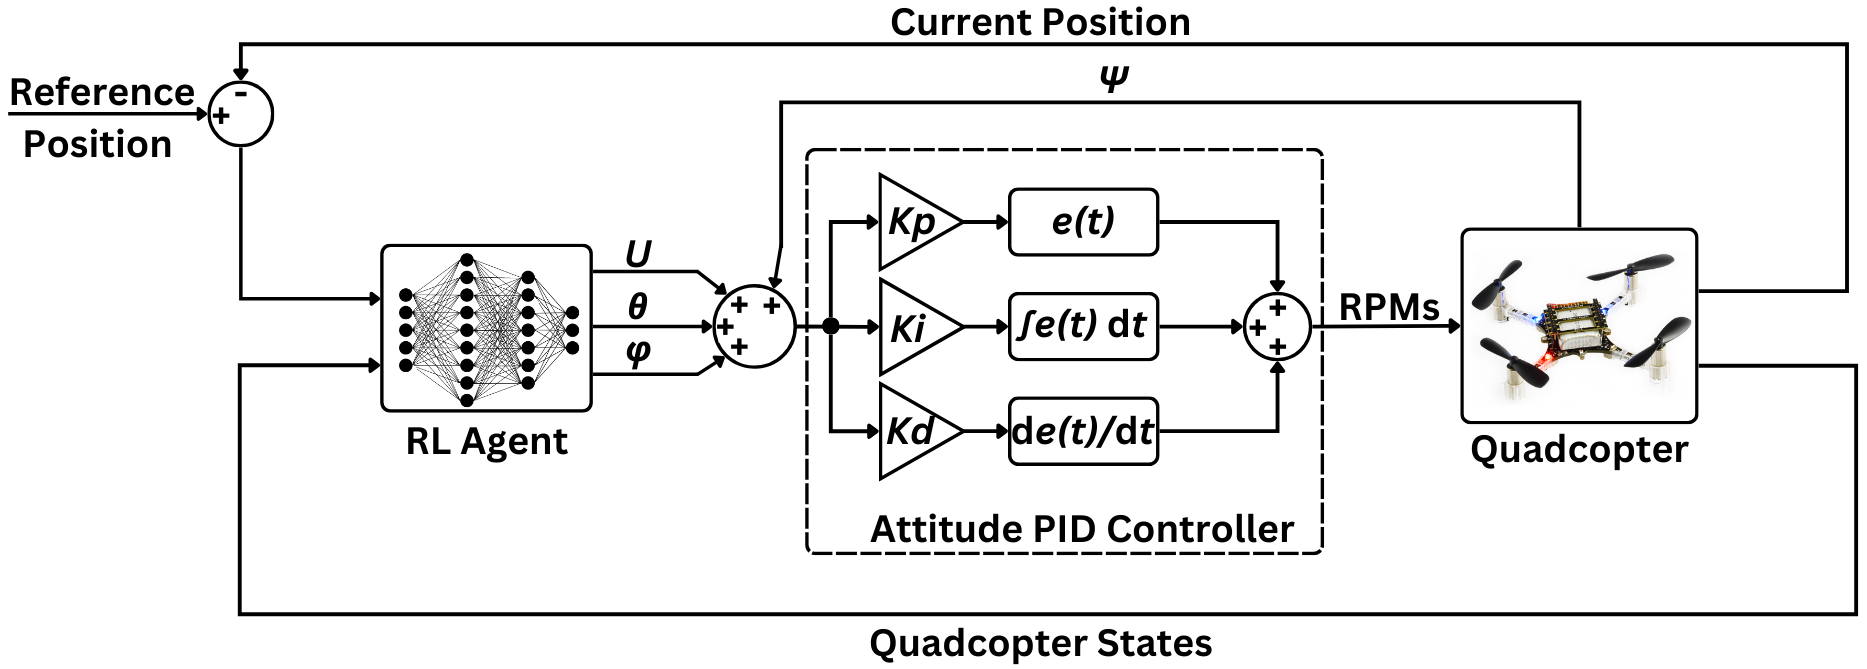
\includegraphics[width=1\linewidth]{Images/mahran.png}
            \caption{Block Diagram of the Position Controller for the Quadcopter}
            \label{mahran_cont}
    \end{figure}
     The agent takes the same input as the previous agent and then sends the calculated action along with the current yaw from the quadcopter to the attitude PID controller which then maps the input values to the desired RPMs. This technique ensures seamless integration with any flight controller with an in-built attitude controller as most known flight controllers don't allow direct manipulation of the motor RPMs and only allow attitude manipulation. \clearpage
    %#######################################################################
       \section{Agent Environment}
    A simple dynamic model of the quadcopter shown in Fig. \ref{drone model} is constructed in the simulation environment using a floating body model with four thrust forces representing the four motors. 
    \begin{figure}[H]
            \centering
            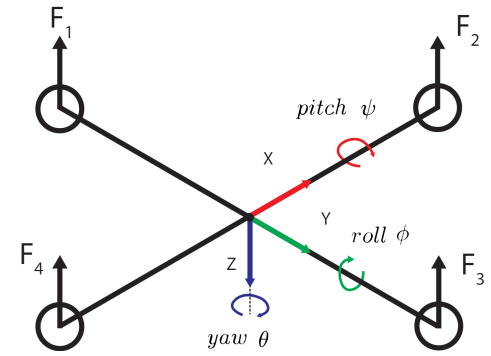
\includegraphics[width=0.5\linewidth]{Images/drone.png}
            \caption{Quadcopter Model Used in Training Environment \cite{mazen}}
            \label{drone model}
    \end{figure}
    Because Model-Free RL is used, an explicit model of the environment is not necessary for the agent to function. The model presented servers as the environment that the agent interacts with. The same environment is used for both path-following and position controllers.
    %################################################
    \section{Network Structure}
     TD3 and SAC were selected due to their effectiveness in continuous control tasks and due to each algorithm inheriting the required policy type for the research. The selected neural network architecture for all networks of the two algorithms consists of two hidden layers with 400 and 300 nodes each, one input layer, and an output layer with one output for the critic and three or four outputs for the actor of the position or path-following controller respectively. LeakyReLU activation functions are used in both hidden layers. Both the path-following and position controller agents have the same architecture.\clearpage
     %#################################
    \section{Stable-baselines3}
    The learning algorithm was implemented using the Stable-baselines3 (SB3) library. SB3 offers various RL algorithms implementations including the SAC and TD3 algorithms. The algorithms are built on the PyTorch platform which enables powerful implementations of the various algorithms. SB3 library can be integrated with OpenAI gym environments which enables easy RL algorithm training. Using the same library for the SAC and TD3 implementations ensures a fair comparison between the two algorithms.
    %#################################
    \section{Simulation Environment}
    Gym-pybullet-drones was used as the simulation environment. The project is built on top of the open-source PyBullet physics engine, which is well-known for its simple user interface and ability to work with a wide range of Python libraries including SB3. PyBullet's rendering engine uses less GPU power than other renderers, which allows for quicker testing and training progress tracking. Its smooth interaction with the OpenAI Gym API further simplifies and increases experimentation by simplifying the testing of different reinforcement learning methods. A comparison between different simulators is shown in Table \ref{simulators}.
    \begin{table}[H]
    \centering
    \begin{adjustbox}{max width=\textwidth}
    \begin{tabular}{lllll}
    \hline
    & \textbf{Gym-pybullet-drones} \cite{pybullet} & \textbf{Flightmare} \cite{flightmare} & \textbf{Airsim} \cite{Airsim} & \textbf{CrazyS} \cite{crazys}\\
    \midrule
    Physics Engine & Pybullet & $Ad hoc$ & PhysX & Gazebo \\
    Rendering Engine & OpenGL3 & Unity & UE4 & OGRE \\
    Language & Python & C++ & C++ & C++ \\
    Synchro./Steppable Physics \& Rendering & \textbf{Yes} & \textbf{Yes} & No & \textbf{Yes} \\
    RGB, Depth, and Segmentation Views & \textbf{Yes} & \textbf{Yes} & \textbf{Yes} & No segmentation \\
    Multiple Vehicles & \textbf{Yes} & \textbf{Yes} & \textbf{Yes} & No \\
    \textit{Gym} API & \textbf{Yes} & W/o Vision & No & No \\
    Multi-agent \textit{Gym}-like API & \textbf{Yes} & No & No & No \\
    \hline
    \end{tabular}
    \end{adjustbox}
    \caption{A Comparison Between the Different Leading Simulation Environments \cite{pybullet}}
    \label{simulators}
    \end{table}\clearpage
    %###################################
    \section{Hyperparameters}
    The effectiveness of any RL algorithm is strongly connected to its hyperparameters, where even little adjustments can result in significant changes in performance outcomes. After tuning the parameters with trial and error, the hyperparameters that were used for the both agents are shown in Table \ref{hyper}.
    \begin{table}[H]
    \centering
    \begin{tabular}{lll}
    \hline
    Symbol & Description & Value \\
    \hline
    $\alpha$ & Learning rate & $0.0007$ \\
    $B$ & Size of the replay buffer &  $1,000,000$\\
    $-$& Steps before learning starts  & $10,000$ \\
    $N$ & Minibatch size & $256$ \\
    $\tau$ & Update coefficient  & $0.005$ \\
    $\gamma$ & Discount factor & $0.99$ \\
    $-$ & Training frequency  & $1$ episode  \\
    $\sigma_{t}$ & Target policy noise  & $0.2$ \\
    $\sigma_{a}$ & Exploration noise  & $0.2$ \\
    $-$ & Target noise clip & $0.5$ \\
    $f$ & Agent frequency  & $50$ Hz \\
    $t_{max}$  & Maximum steps of one episode  & $502$ \\
    \hline
    \end{tabular}    
    \caption{Hyperparameters Used for the Deterministic and Stochastic Agents}
    \label{hyper}
    \end{table}
    A small learning rate was chosen to ensure stability while training. A high discount factor encourages the agent to favor future rewards over immediate ones. A normal action noise with a standard deviation of 0.2 was added to encourage exploration over exploitation.\\
    The same set of hyperparameters is used across the two algorithms to ensure a fair comparison between the two algorithms. However, the SAC introduces an extra parameter which is the entropy coefficient. The entropy coefficient was set to an 'auto' value which means the agent learns the optimal entropy value while training and changes the value according to the training demands.\clearpage
    %###################################
    \section{Observation \& Action Space}
    The observation space of both controllers consists of 12 inputs. The current orientation of the quadcopter, current linear and angular velocities, and the difference between the quadcopter's position and the target position. The Observation space is shown in Eq. \ref{obs}.
    \begin{equation}
        S = [\phi, \theta, \psi, v_{\textit{x}}, v_{\textit{y}}, v_{\textit{z}}, \omega_{\textit{x}}, \omega_{\textit{y}}, \omega_{\textit{z}},\Delta x, \Delta y, \Delta z]
        \label{obs}
    \end{equation}
    The action space for both agents and controllers is continuous. The actions of the path-following controller represent the four RPMs of the quadcopter’s rotors. The actions are normalized as shown in Eq. \ref{rpm} and Eq. \ref{i}:
    \begin{equation}
        a_{i} \in [-1, 1]
        \label{rpm}
    \end{equation} 
    \begin{equation}
        i \in [1, 4]
        \label{i}
    \end{equation}
    The action space of the position controller on the other hand consists of only three actions presented as the precentage of overall vertical thrust along the quadcopter's $z$-axis, the desired roll angle, and the desired pitch angle as shown in Eq. \ref{pid}. The actions are normalized to the range [-1, 1].
        \begin{equation}
        a = [U_{1}, \theta, \phi]
        \label{pid}
    \end{equation} \clearpage
    %###################
    \section{Reward Function}
    To encourage the agent and achieve the intended goals, a reward function is essential. There are two types of reward functions in RL: sparse rewards and dense rewards. Sparse rewards are given to the agent only in terminal states. Because sparse rewards are typically associated with "rare" states, they carry high values that impact the agent's sense of state values. Dense rewards, on the other hand, are given to the agent at every step and are usually of lower value. Dense rewards have the potential to generate bias because, in contrast to sparse rewards, which rarely offer feedback on successes or failures, they give the agent insights into the environment. Given the continuous nature of the environment states in this case, dense reward functions were used for the agent. The reward function was derived from the literature \cite{Mokhtar}.
    \begin{equation}
    r = \frac{1}{a \text{  }* \text{  }||\vec{e}_{k}||_{2}} + \frac{a}{\sqrt{2\pi \sigma^2}} e^{-0.5(\frac{||\vec{e}_{k}||_{2}}{\sigma})^2}
    \label{reward}
    \end{equation}
    \begin{equation}
    ||\vec{e}_{k}||_{2} = \sqrt{\Delta x^2 + \Delta y^2 + \Delta z^2}
    \label{ec}
    \end{equation}
    The reward function presented in Eq. \ref{reward} consists of two different parts. The first part is a rational function with $a = 7$ and $||\vec{e}_{k}||_{2}$ representing the Euclidean distance as shown in Eq. \ref{ec}. This part is responsible for tracking the stable hovering of the quadcopter. The second part is a normal distribution function with a standard deviation of 0.5 responsible for tracking the quadcopter with each step closer to the target yields a higher positive reward. The same reward function was used for the position and path-following controllers.\clearpage
    %###################################
    \section{Training Limits \& Goal}
    Four different trainings are presented in this thesis with each controller being trained twice. The goal of each training is shown below.
\begin{enumerate}[label={\textit{\alph*)}}]
    \item{\textit{Path-following Agent Training:}}
    \begin{enumerate}[label={\textit{\arabic*.}}]
    \item \textit{Small State Space Training:}\\
    The goal of this training is to train the agent to start from any random position and reach the fixed target of [0, 0, 1]. To fully test the deterministic and stochastic algorithms, the agents were trained using two different state spaces, a large and small one. The first training had the initial position change each episode by choosing a random value from the following values:
    \begin{itemize}
        \item \(x\) and \(y\) \(\in\) [-0.5, 0.5]
        \item \(z\) \(\in\) [0.5, 1.5]
    \end{itemize}
    \item \textit{Large State Space Training:}\\
    The second training increased the state space to the following values:
    \begin{itemize}
        \item \(x\) and \(y\) \(\in\) [-2.5, 2.5]
        \item \(z\) \(\in\) [0.2, 2.5]
    \end{itemize}
    The two different state spaces were used to fully test the ability of each algorithm in covering and learning the entirety of the state space and compare their results.
    \end{enumerate}
    \item{\textit{Position Controller Agent Training:}}
    \begin{enumerate}[label={\textit{\arabic*.}}]
        \item \textit{Stabilization Training:}\\
    The goal of this training is similar to that of the path-following agent. The quadcopter starts from a random position each episode and tries to reach the fixed target of [0, 0, 1]. The initial position is chosen randomly from the following values:
    \begin{itemize}
        \item \(x\) and \(y\) \(\in\) [-1.5, 1.5]
        \item \(z\) \(\in\) [0, 2]
    \end{itemize}
   \clearpage
    \item \textit{Trajectory Tracking Training:}\\
    The goal of this training is for the quadcopter to start from a random position each episode and try to reach a random target. The initial position and target are changed randomly in each episode with the initial position having the same values of the stabilization training and the target position was chosen randomly from this set of values:
    \begin{itemize}
        \item \(x\) and \(y\) \(\in\) [-1.3, 1.3]
        \item \(z\) \(\in\) [0.2, 1.9]
    \end{itemize}
    The random initial position and random target encourage the agent to reach any point in the state space from any position the quadcopter is in.
    \end{enumerate}
    \item{\textit{Training Limits:}}\\
    Several limits were included where the episode would end if the quadcopter crashed or left a bounded area to speed up the simulation. The same limits were used across the four trainings.
    \begin{itemize}
        \item \(\phi\) or \(\theta\) or \(\psi\) \(>\) \(\pi/2\)
        \item \(x\) or \(y\) \(>\) 3
        \item \(z\) \(>\) 3 or \(z\) \(<\) 0.2
    \end{itemize}
    \end{enumerate}
    %#################################
    \section{Training Setup}
    The training procedure followed the conditions and parameters demonstrated above. The training platform was a CrazeFlie2.0 Drone model set up in an X layout in the gym-pybullet-drones environment. The PyTorch library, which smoothly incorporates CUDA for simplified device selection, was used to construct ML algorithms, while the Stable-Baselines3 library made it easier to implement the TD3 and SAC algorithms. TensorBoard was used to track progress. Training was accelerated by using NVIDIA CUDA on a GeForce RTX 3070 GPU, which allowed for the quick completion of multiple episodes.
    %############################
    

